\chapter{STG}
\label{ch:stg}

% Uvod: Imperativni vs funkcijski programski jeziki
Glede na paradigmo delimo programske jezike na imperativne in deklarativne. Imperativni jeziki, kot so npr. C, Rust, Python, \dots, iz vhodnih podatkov izračunajo rezultat s pomočjo stavkov, ki spreminjajo notranje stanje programa. Ukazi oziroma stavki podrobno opisujejo kako naj se program izvaja, in jih je zato nekoliko lažje prevesti v strojne ukaze, ki jih zna izvajati procesor. Pri deklarativnem programiranju pa je program podan kot višjenivojski opis želenega rezultata, ki ne opisuje dejanskega poteka programa. Med deklarativne jezike štejemo npr. SQL, katerega program je opis podatkov, ki jih želimo pridobiti in kako jih želimo manipulirati, ne da bi podrobno opisovali kako naj sistem izvede te operacije.

% Funkcijski programski jeziki
Med deklarativne programske jezike pa spadajo tudi funkcijski. Ti za osnovno operacijo nad podatki smatrajo čisto (angl. pure) funkcijo, tj. funkcijo, ki za izračun svoje vrednosti uporablja le vrednosti svojih argumentov, ne pa tudi drugega globalnega stanja. Prednost čistih funkcij je, da bodo enaki vhodi vedno producirali enake izhode, kar omogoča optimizacijo programa s pomočjo memoizacije. Osnovni primitiv je v takih jezikih funkcija, kar pomeni, da jih je mogoče prirediti v spremenljivke, jih uporabiti kot argumente in rezultate drugi funkcij. Čist funkcijski program lahko tako opišemo kot kompozicijo čistih funkcij, ki vhod preslikajo v izhod.

Poleg čistih funkcij je ena izmed ključnih značilnosti mnogih funkcijskih jezikov tudi leni izračun (angl. lazy evaluation). Leni izračun je strategija računanja vrednosti izrazov, pri kateri se vrednost izraza ne izračuna takoj, ko je definiran, ampak šele, ko je njegova vrednost dejansko potrebna. Ta pristop je tesno povezan z deklarativno naravo funkcijskega programiranja in omogoča pisanje bolj modularne in učinkovite kode.

V poglavju se bomo podrobneje posvetili \textit{lenim} funkcijskim jezikom, podrobneje bomo definirali leni izračun, ter predstavili Haskell, jezik, ki temelji na čistih funkcijah in lenosti. Podrobneje bomo opisali potek prevajanja jezika v vmesni jezik imenovan STG in opisali delovanje abstraktnega STG stroja, ki ga zna izvajati.

\section{Leni izračun}
\label{sec:leni-izracun}

% Kaj je semantika, primerjava stroge in nestroge semantike
Semantika programskega jezika opisuje pravila in principe, ki določajo kako se programi izvajajo. Semantiko za izračun izrazov v grobem delimo na strogo (angl. strict) in nestrogo (angl. non-strict). Večina programskih jezikov pri računanju izrazov uprablja strogo semantiko, ki določa, da se izrazi izračunajo \textit{takoj, ko so definirani}. Nasprotno, nestroga semantika določa, da se izrazi izračunajo šele, ko so dejansko potrebni za nadaljnjo obdelavo, oziroma se sploh ne izračunajo, če niso potrebni.

% Prevladovanje stroge semantike
Večina današnjih programskih jezikov temelji na strogi semantiki. Mednje spadajo tako imperativni jeziki, kot so npr. C, Rust, Python, kot tudi funkcijski programski jeziki kot sta npr. Ocaml in Lisp. Jezikov, ki temeljijo na nestrogi semantiki je bistveno manj, med njimi npr. jeziki Haskell, Miranda in Clean.

% Primer
\begin{code-box}{haskell}{Haskell}
konjunkcija :: Bool -> Bool -> Bool
konjunkcija p q =
	case p of
		False -> False
		True -> q
\end{code-box}

Kot primer si oglejmo razliko pri evalvaciji izraza izraza \texttt{konjunkcija False ((1 / 0) == 0)}. Jeziki, ki temeljijo na strogi semantiki ob klicu funkcije najprej izračunajo vrednosti argumentov. Ker pride pri izračunu drugega argumenta do napake, se izvajanje programa tukaj ustavi. Pri jezikih z nestrogo semantiko pa se ob klicu funkcije ne izračunajo vrednosti argumentov, temveč se računanje izvede šele takrat, ko je vrednost dejansko potrebovana. Ker je prvi argument pri klicu funkcije \texttt{False}, funkcija drugega argumenta ne evalvira in tako je rezultat klica vrednost \texttt{False}.

% Formalizacija stroge in nestroge semantike
Če semantika jezika dopušča izračun vrednosti izraza, kljub temu, da njegovi podizrazi nimajo vrednosti, jo imenujemo za strogo semantiko. Bolj formalno lahko uvedemo vrednost $\bot$, ki jo imenujemo tudi dno (angl. bottom) in predstavlja vrednosti izrazov, katerim ni mogoče izračunati normalne oblike. Če izraza \textit{expr} ne moremo evalvirati, lahko tako zapišemo kar $\textbf{eval}(expr) = \bot$. Za funkcijo enega argumenta pravimo, da je \textit{stroga}, če velja naslednji pogoj.

$$ f \: \bot = \bot $$

Za stroge funkcije torej velja, da če se argument ne bo izračunal, se tudi rezultat klica funkcije z argumentom ne  bo evalviral. Če funkcija ni stroga, pravimo da je nestroga.

% Strogi izračun
Strogi izračun (angl. eager evaluation) je način implementacija stroge semantike, pri katerem so vrednosti argumentov izračunane pred klicem funkcije. Strogemu izračunu zato pravimo tudi [TODO] (angl. call by value). Obratno, je leni izračun (angl. lazy evaluation) način implementacije nestroge semantike. Pri lenem izračunu izrazi niso evalvirani kadar jih \textit{priredimo} spremenljivki, temveč je njihov izračun odložen na poznejši čas, kadar je vrednost izraza dejansko potrebovana. Ker se izračun izvaja po potrebi po vrednosti, to strategijo imenujemo izračun po potrebi (angl. call by need).

% Prednosti in slabosti
Ena izmed slabosti strogega izračuna je v tem, da klicana funkcija morebiti argumenta sploh ne potrebuje, kar pomeni, da se je ob klicu funkcije vrednost argumenta izračunala brez potrebe. Prednost strogega izračuna pa je v tem, da je izvajanje bolj predvidljivo, saj za razliko od lenega izračuna natančno vemo kdaj se bodo argumenti evalvirali. Prednost lenega izračuna pa leži v tem, da so argumenti evalvirani \textit{največ enkrat}. Če namreč argument v telesu funkcije ni nikoli uporabljen, potem tudi ne bo nikoli izračunan. Če pa je uporabljen, bo njegova vrednost izračunana \textit{enkrat} in memozirana v vseh preostalih uporabah. Slabost lenega izračuna pa je v tem, da ga je težje implementirati in da se navadno izvaja počasneje od jezikov s strogim izračunom.

% TODO: Reduction order - normal vs leftmost outmost

\subsubsection{Redukcija grafa}

% Razlika med imperativnimi in funkcijskimi jeziki - izvajanje
Zgodnejši programski jeziki so bili namenjeni neposrednemu upravljanju ra\-ču\-nal\-ni\-ka in so kot taki precej odražali delovanje računalniške arhitekture na kateri so se izvajali~\cite{10.1145/72551.72554}. Funkcijski programski jeziki omogočajo večji nivo abstrakcije, so bolj podobni matematični notaciji in posledično tudi bolj primerni za dokazovanje pravilnosti programov. Višji nivo abstrakcije pa pomeni, da jih je težje prevajati oziroma izvajati na današnji računalniški arhitekturi. Ena izmed ovir pri implementaciji lenega izračuna je učinkovito upravljanje z odloženimi izrazi (angl. thunks) in zagotavljanje, da se ti izrazi izračunajo le, ko so resnično potrebni.

% Kako implementiramo leni izračun?
Leni izračun najpogosteje implementiramo s pomočjo redukcije gra\-fa~\cite{peyton1987implementation, 10.1145/72551.72554}. Pri tej metodi prevajalnik na pomnilniku najprej sestavi abstraktno sintaksno drevo programa, kjer vozlišča predstavljajo aplikacije funkcij oziroma operacije nad podatki, njihova podvozlišča pa odvisnosti med njimi. V procesu \textit{redukcije}, se sintaksno drevo obdeluje z lokalnimi transformacijami, ki ga predelujejo, dokler ni dosežena končna oblika, tj. dokler ni izračunan rezultat programa. Pri tem se sintaksno drevo zaradi deljenja izrazov (angl. expression sharing) navadno spremeni v usmerjen graf.

Slika \ref{fig:redukcija-aplikacije-pred} prikazuje abstraktno sintaktično drevo izraza $(\lambda x \, . \, \textsc{not} \; x) \; \text{True}$. Aplikacija funkcij je predstavljena z vozliščem @, ki vsebuje dva podizraza: funkcijo, ki se bo izvedla in njen argument. V tem primeru je funkcija anonimni lambda izraz $(\lambda x \, . \, \textsc{not} \; x)$, ki sprejme en argument. Pri redukciji, se vse uporabe parametra $x$ zamenjajo z vrednostjo argumenta \texttt{True}. Slika \ref{fig:redukcija-aplikacije-po} prikazuje drevo po redukciji. Ker se je v funkciji argument $x$ pojavil le enkrat, je rezultat redukcije še vedno drevo.

\begin{figure*}[ht]
	\centering
	\begin{subfigure}[b]{0.45\textwidth}
		\centering
		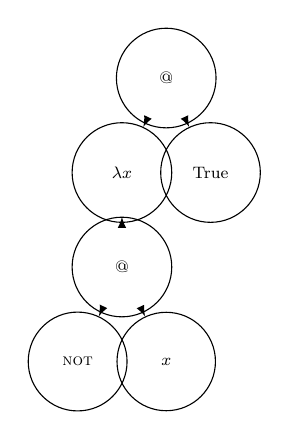
\begin{tikzpicture}[
			scale=0.75, transform shape,
			main/.style = {draw, circle},
			edge from parent/.style={draw,-latex},
			level distance=1.6cm,align=center,text width=0.75cm,
			]
			\node[main] (root) {@}
			child { node[main] {$\lambda x$}
				child { node[main] {@}
					child { node[main] {\textsc{not}} }
					child { node[main] {$x$} }
				}
			}
			child { node[main] {True} };
		\end{tikzpicture}
		\subcaption{Abstraktno sintaksno drevo \textit{pred} redukcijo}
		\label{fig:redukcija-aplikacije-pred}
	\end{subfigure}%
	\hfill
	\begin{subfigure}[b]{0.45\textwidth}
		\centering
		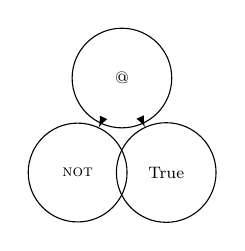
\begin{tikzpicture}[
			scale=0.75, transform shape,
			main/.style = {draw, circle},
			edge from parent/.style={draw,-latex},
			level distance=1.6cm,align=center,text width=0.75cm,
			]
			\node[main] (root) {@}
			child { node[main] {\textsc{not}} }
			child { node[main] {True} };
		\end{tikzpicture}
		\subcaption{Abstraktno sintaksno drevo \textit{po} redukciji}
		\label{fig:redukcija-aplikacije-po}
	\end{subfigure}
	\caption{Redukcija grafa izraza $(\lambda x \, . \, \textsc{not} \; x) \; \texttt{True}$}
	\label{fig:redukcija-aplikacije}
\end{figure*}

Slika \ref{fig:redukcija-dvojne-aplikacije} prikazuje en korak redukcije abstraktnega sintaksnega drevesa izraza $(\lambda x \, . \, \textsc{and} \; x \; x) \; (\textsc{not} \; \texttt{True})$. Po enem koraku redukcije sintaksnega telesa, se \textit{vse uporabe} parametra $x$ zamenjajo z njegovo vrednostjo. Ker je takih pojavitev več, pa rezultat ni več drevo, temveč acikličen usmerjen graf. Na pomnilniku tak izraz predstavimo z dvema kazalcema na isti objekt. Ko se objekt prvič izračuna, se vrednost objekta na pomnilniku posodobi z izračunano vrednostjo. Ob vseh nadaljnjih uporabah argumenta, tako ne bo potrebno še enkrat računati njegove vrednosti, s čemer dosežemo, da bo vsak argument izračunan največ enkrat. 

\begin{figure*}[ht]
	\centering
	\begin{subfigure}[b]{0.45\textwidth}
		\centering
		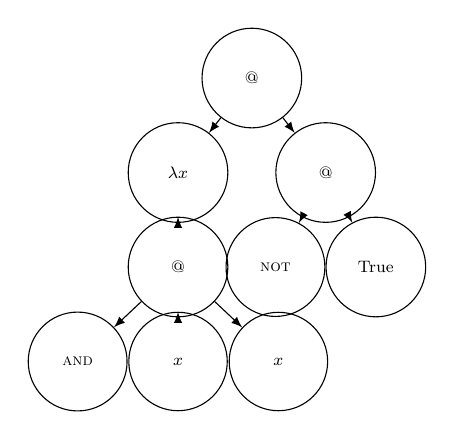
\begin{tikzpicture}[
			scale=0.75, transform shape,
			main/.style = {draw, circle},
			edge from parent/.style={draw,-latex},
			level distance=1.6cm,align=center,text width=0.75cm,
			level 1/.style={sibling distance=2.5cm},
			level 2/.style={sibling distance=1.7cm},
			]
			\node[main] (root) {@}
			child { node[main] {$\lambda x$}
				child { node[main] {@}
					child { node[main] {\textsc{and}} }
					child { node[main] {$x$} }
					child { node[main] {$x$} }
				}
			}
			child { node[main] {@}
				child { node[main] {\textsc{not}} }
				child { node[main] {True} }
			};
		\end{tikzpicture}
	\end{subfigure}%
	\hfill
	\begin{subfigure}[b]{0.45\textwidth}
		\centering
		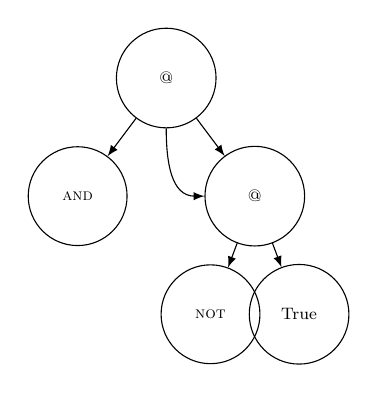
\begin{tikzpicture}[
			scale=0.75, transform shape,
			main/.style = {draw, circle},
			edge from parent/.style={draw,-latex},
			level distance=2cm,align=center,text width=0.75cm,
			]
			\node[main] (root) {@}
			child { node[main] {\textsc{and}} }
			child { edge from parent[draw=none] }
			child { node[main] (argument) {@}
				child { node[main] {\textsc{not}} }
				child { node[main] {True} }
			};
			\draw[-latex] (root) to[out=-90, in=180, looseness=1.1] (argument);
		\end{tikzpicture}
	\end{subfigure}
	\caption{Redukcija grafa izraza $(\lambda x \, . \, \textsc{and} \; x \; x) \; (\textsc{not} \; \texttt{True})$}
	\label{fig:redukcija-dvojne-aplikacije}
\end{figure*}

Slika \ref{fig:funkcija-y} prikazuje dve možni implementaciji ciklične funkcije $Y \; f = f \; (Y \; f)$. Za razliko od primerov na slikah \ref{fig:redukcija-aplikacije} in \ref{fig:redukcija-dvojne-aplikacije}, pri katerih je bilo reducirano sintaktično drevo še vedno usmerjen acikličen graf, pa temu pri funkciji $Y$ ni več tako. Funkcija $Y$ je namreč rekurzivna, kar pomeni, da se sama pojavi kot vrednost svojega argumenta. Na sliki \ref{fig:funkcija-y-kot-prosta-spremenljivka} je funkcija $Y$ implementirana s pomočjo acikličnega grafa, a v svojem telesu vseeno dostopa do proste spremenljivke $Y$, zaradi česar obstaja na pomnilniku cikel. Na sliki \ref{fig:funkcija-y-kot-cikel} je funkcija implementirana neposredno s pomnilniškem ciklu, kjer je vrednost argumenta kar vozlišče samo.

\begin{figure*}[ht]
	\centering
	\begin{subfigure}[b]{0.45\textwidth}
		\centering
		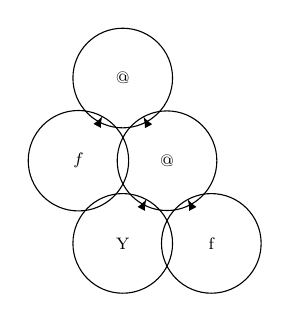
\begin{tikzpicture}[
			scale=0.75, transform shape,
			main/.style = {draw, circle},
			edge from parent/.style={draw,-latex},
			level distance=1.4cm,align=center,text width=0.75cm,
			]
			\node[main] (root) {@}
			child { node[main] {$f$} }
			child { node[main] {@}
				child { node[main] {Y} }
				child { node[main] {f} }
			};
		\end{tikzpicture}
		\subcaption{Funkcija $Y$ implementirana z uporabo proste spremenljivke}
		\label{fig:funkcija-y-kot-prosta-spremenljivka}
	\end{subfigure}%
	\hfill
	\begin{subfigure}[b]{0.45\textwidth}
		\centering
		\begin{tikzpicture}[
			scale=0.75, transform shape,
			main/.style = {draw, circle},
			edge from parent/.style={draw,-latex},
			level distance=1.4cm,align=center,text width=0.75cm,
			]
			\node[main] (root) {@}
			child { node[main] {$f$} }
			child { node (right) {} edge from parent[draw=none] };
			\coordinate [above=0.6cm of root] (above-root);
			\coordinate [right=0.4cm of right] (right-of-right);
			\coordinate (intermediate) at (right-of-right |- above-root);
			\draw[-latex] (root) -- (right.center) -- (right-of-right) -- (intermediate) -- (above-root) -- (root.north);
		\end{tikzpicture}
		\subcaption{Funkcija $Y$ implementirana kot cikličen usmerjen graf}
		\label{fig:funkcija-y-kot-cikel}
	\end{subfigure}
	\caption{Graf funkcije $Y \; f = f \; (Y \; f)$}
	\label{fig:funkcija-y}
\end{figure*}

\subsubsection{Zapis grafa na pomnilniku}

\begin{figure*}[ht]
	\centering
	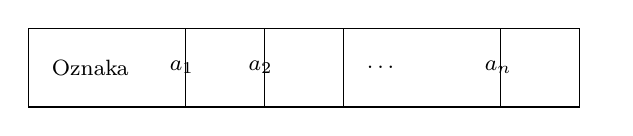
\begin{tikzpicture}[
		% Popravi vertikalno pozicioniranje teksta
		% https://tex.stackexchange.com/a/133237/324113
		verticalalign/.append style={font=\vphantom{Ag}}
		]
		\draw[verticalalign] (0,0) rectangle ++(2,1) node[midway] {Oznaka};
		\draw[verticalalign] (2,0) rectangle ++(1,1) node[midway] {$a_1$};
		\draw[verticalalign] (3,0) rectangle ++(1,1) node[midway] {$a_2$};
		\draw[verticalalign] (4,0) rectangle ++(2,1) node[midway] {$\dots$};
		\draw[verticalalign] (6,0) rectangle ++(1,1) node[midway] {$a_n$};
	\end{tikzpicture}
	\caption{Pomnilniška predstavitev vozlišča grafa}
	\label{fig:shema-vozlisca-pomnilnik}
\end{figure*}

\begin{figure*}[ht]
	\centering
	\begin{tikzpicture}
		\draw (0,0) rectangle ++(1,1) node[midway] {\textbf{@}};
		\draw (1,0) rectangle ++(2,1) node[midway] (and) {};
		\draw (3,0) rectangle ++(2,1) node[midway] (and-arg1) {};
		\draw (5,0) rectangle ++(2,1) node[midway] (and-arg2) {};
		
		\draw (0,-2) rectangle ++(1,1) node[midway] (app-not) {\textbf{@}};
		\draw (1,-2) rectangle ++(2,1) node[midway] (not) {};
		\draw (3,-2) rectangle ++(2,1) node[midway] {\texttt{0b1}};
		
		\node (above-and) at (2,2) {\textsc{and}};
		\node (below-not) at (2,-3) {\textsc{not}};
		
		\draw[] (and-arg1) -- ++(0,-1);
		\draw[-latex] (and-arg2) -- ++(0,-1) -- ++(-7,0) -- ++(0,-1) -- ++(1,0);
		
		\draw[-latex] (and) -- ++(0,1);
		\draw[-latex] (not) -- ++(0,-1);
		% \draw[-latex] (and) -- (above-and);
	\end{tikzpicture}
	\caption{Predstavitev izraza $\textsc{and} \; (\textsc{not} \; \texttt{True}) \; (\textsc{not} \; \texttt{True})$ na pomnilniku}
	% \label{fig:}
\end{figure*}

Leno evalvacijo najpogosteje implementiramo s pomočjo zakasnitev (angl. thunks). Te so na pomnilniku predstavljene kot kazalec na kodo, ki izračuna njihovo vrednost. Ob evalvaciji zakasnitve se najprej izračuna njihova vrendost, izračunano vrednost pa se shrani v struktro na pomnilniku, da je ob naslednji evalvaciji ni potrebno ponovno računati. Na tak način se z nestrogo semantiko doseže, da se vsak izraz izračuna \textit{največ enkrat}. Če se argument ne pojavi nikjer v telesu funkcije, se zakasnitve nikoli ne računa, če pa se v telesu pojavi večkrat, se vrednost izračuna enkrat, za vsako nadaljno evalvacijo argumenta pa se preprosto vrne vrednost shranjeno na pomnilniku.

% TODO: Omenimo še, da je pri lenem izračunu zelo težko predvideti koliko prostora bo program porabil, kar pa ni velik problem pri imperativnih jezikih.
% TODO: Problem: Funkcije so first-class-citizens, kar pomeni, da je potrebno nekoliko več razmisliti o predstavitvi funkcij na pomnilniku.

% Povezava z naslednjim poglavjem
V nadeljevanju se bomo osredotočili na delovanje prevajalnika GHC (angl. Glasgow Haskell compiler), ki izvorno kodo napisano v programskem jeziku Haskell prevede v strojno kodo. Pri prevajanju se program transformira v več različnih vmesnih predstavitev (angl. intermediate representation), mi pa se bomo v magistrskem delu osredotočili predvsem na vmesno kodo imenovano STG jezik (angl. Spineless tagless G-Machine language), katerega delovanje bomo podrobneje opisali v razdelku \ref{sec:stg-jezik}.


\section{Prevajalnik GHC}
\label{sec:prevajalnik-ghc}

Prevajalnik GHC (angl. Glasgow Haskell compiler) prevajanje iz izvorne kode v programskem jeziku Haskell v strojno kodo izvaja v več zaporednih fazah oziroma modulih. Vsaka faza kot vhod prejme izhod prejšnje, nad njim izvede določeno transformacijo in rezultat posreduje naslednji fazi. Faze glede na njihovo funkcijo v grobem delimo na tri dele. V prednjem delu (angl. front-end) se nad izvorno kodo najprej izvede leksikalna analiza, pri kateri se iz toka znakov, ki predstavljajo vhodni program pridobi abstraktno sintaktično drevo (angl. abstract syntax tree). Nad drevesom se izvede še zaporedje semantičnih analiz pri katerih se preveri ali je program pomensko pravilen. Sem sodi razreševanje imen, pri kateri se razreši vsa imena spremenljivk iz uvoženih modulov v programu in preveri ali so vse spremenljivke deklarirane pred njihovo uporabo. Izvede se še preverjanje tipov, kjer se za vsak izraz izpelje njegov najbolj splošen tip in preveri ali se vsi tipi v programu ujemajo.

\begin{figure}[h]
	\centering
	\begin{tikzpicture}
		\tikzset{
			every node/.append style={text width=1.4cm,execute at begin node=\setlength{\baselineskip}{1em},font=\footnotesize},
			block/.style={draw,rectangle,text width=2cm,align=center,minimum height=1cm,minimum width=2cm},
		}
		
		% Srednji del prevajalnika
		\node[block] (optimizacija) {Optimizacija};
		\node[coordinate, left=2.6cm of optimizacija] (center-levo) {};
		\node[coordinate, right=2.6cm of optimizacija] (center-desno) {};
		
		% Prednji del prevajalnika
		\node[block, above=0.55cm of center-levo] (semanticna-analiza) {Semantična analiza};
		\node[block, above=0.55cm of semanticna-analiza] (razclenjevanje) {Razčlen\-je\-van\-je};
		\node[block, below=0.55cm of semanticna-analiza] (izpeljava-tipov) {Izpeljava tipov};
		\node[block, below=0.55cm of izpeljava-tipov] (razsladenje) {Razsladenje};
		
		% Zadnji del prevajalnika
		\node[block, above=0.55cm of center-desno] (stg-to-cmm) {Izbira \texttt{C--} ukazov};
		\node[block, above=0.55cm of stg-to-cmm] (core-to-stg) {Izbira STG ukazov};
		
		% Moznosti prevajanja C-- -> strojna koda
		\node[block, minimum height=0.6cm, below=0.9cm of stg-to-cmm] (neposredno) {Neposredno};
		\node[block, minimum height=0.6cm, below=0.3cm of neposredno] (gcc) {GCC};
		\node[block, minimum height=0.6cm, below=0.3cm of gcc] (llvm) {LLVM};
		
		% 
		\node[coordinate, left=0.4cm of neposredno.west] (levo-od-neposredno) {};
		\node[coordinate, left=0.4cm of gcc.west] (levo-od-gcc) {};
		\node[coordinate, left=0.4cm of llvm.west] (levo-od-llvm) {};
		\draw[-] (levo-od-neposredno) -- (levo-od-gcc) -- (levo-od-llvm);
		\draw[->] (levo-od-neposredno) -- (neposredno);
		\draw[->] (levo-od-gcc) -- (gcc);
		\draw[->] (levo-od-llvm) -- (llvm);
		
		\node[coordinate, right=0.4cm of neposredno.east] (desno-od-neposredno) {};
		\node[coordinate, right=0.4cm of gcc.east] (desno-od-gcc) {};
		\node[coordinate, right=0.4cm of llvm.east] (desno-od-llvm) {};
		\draw[-] (desno-od-neposredno) -- (desno-od-gcc) -- (desno-od-llvm);
		\draw[-] (neposredno) -- (desno-od-neposredno);
		\draw[-] (gcc) -- (desno-od-gcc);
		\draw[-] (llvm) -- (desno-od-llvm);
		
		\node[coordinate, below=0.55cm of stg-to-cmm] (pod-stg-to-cmm) {};
		\node[coordinate] at (pod-stg-to-cmm -| levo-od-neposredno) (nad-levo-od-neposredno) {};
		\draw[-] (stg-to-cmm) -- (pod-stg-to-cmm) node[pos=0.5,right] {\scriptsize \texttt{C--}} -- (nad-levo-od-neposredno) -- (levo-od-neposredno) ;
		
		\draw[->] (razclenjevanje) -- (semanticna-analiza) node[pos=0.5,right] {\scriptsize AST};
		\draw[->] (semanticna-analiza) -- (izpeljava-tipov) node[pos=0.5,right] {\scriptsize AST};
		\draw[->] (izpeljava-tipov) -- (razsladenje) node[pos=0.5,right] {\scriptsize AST};
		
		\draw[->] (core-to-stg) -- (stg-to-cmm) node[pos=0.5,right] {\scriptsize STG};
		
		% Puscica "Generator vmesne kode" -> "Optimizacija vmesne kode"
		\node[coordinate, left=0.5cm of optimizacija.west] (levo-od-optimizacija) {};
		\node[coordinate] at (razsladenje -| levo-od-optimizacija) (desno-od-razsladenje) {};
		
		\draw[->] (razsladenje.east) -- (desno-od-razsladenje) -- (levo-od-optimizacija) node[pos=0.5,right] {\scriptsize Core} -- (optimizacija);
		
		% Puscica "Optimizacija vmesne kode" -> "Izbira ukazov"
		\node[coordinate, right=0.5cm of optimizacija.east] (desno-od-optimizacija) {};
		\node[coordinate] at (core-to-stg -| desno-od-optimizacija) (levo-od-izbira-ukazov) {};
		
		\draw[->] (optimizacija) -- (desno-od-optimizacija) -- (levo-od-izbira-ukazov) node[pos=1.0,left,align=right] {\scriptsize Core} -- (core-to-stg);
		
		% Vhodna povezava "Zacetek" -> "Leksikalna analiza"
		\node[coordinate, left=2cm of center-levo] (zacetek) {};
		\node[coordinate, left=0.5cm of razclenjevanje] (levo-od-razclenjevanje) {};
		\node[coordinate] at (zacetek -| levo-od-razclenjevanje) (desno-od-zacetek) {};
		
		\draw[->] (zacetek) -- (desno-od-zacetek) -- (levo-od-razclenjevanje) node[pos=0.2,left,text width=0.9cm] {\scriptsize tok\\znakov} -- (razclenjevanje);
		
		% Koncna povezava
		\node[coordinate, right=2cm of center-desno] (konec) {};
		\node[coordinate] at (konec -| desno-od-neposredno) (levo-od-konec) {};
		\draw[->] (desno-od-neposredno) -- (levo-od-konec) -- (konec) node[pos=1,above] {\scriptsize strojna\\koda};
		
		% Locevalne crte
		\node[coordinate, left=0.25cm of levo-od-optimizacija] (sprednji-del-center) {};
		\node[coordinate, above=3.7cm of sprednji-del-center] (sprednji-del-zgoraj) {};
		\node[coordinate, below=3.2cm of sprednji-del-center] (sprednji-del-spodaj) {};
		\draw[dashed] (sprednji-del-zgoraj) -- (sprednji-del-spodaj) node[pos=0,left=0.2cm,text width=2cm,align=right] {prednji del} node[pos=0,right=0.2cm,text width=2cm] {srednji del};
		
		\node[coordinate, right=0.25cm of desno-od-optimizacija] (zadnji-del-center) {};
		\node[coordinate, above=3.7cm of zadnjif-del-center] (zadnji-del-zgoraj) {};
		\node[coordinate, below=3.2cm of zadnji-del-center] (zadnji-del-spodaj) {};
		\draw[dashed] (zadnji-del-zgoraj) -- (zadnji-del-spodaj) node[pos=0,right=0.2cm,text width=2cm] {zadnji del};
		
	\end{tikzpicture}
	\caption{Pomembnejše faze prevajalnika Glasgow Haskell compiler}
	\label{fig:shema-ghc}
\end{figure}

Bogata sintaksa programskega jezika Haskell predstavlja velik izziv za izdelavo prevajalnikov, saj zahteva natančno prevajanje raznolikih sintaktičnih struktur in konstruktov v strojno kodo. Težavo rešuje zadnji korak prednjega dela prevajalnika, imenovan razsladenje (angl. desugarification). V njem se sintaktično drevo jezika Haskell pretvori v drevo jezika Core, ki je minimalističen funkcijski jezik, osnovan na lambda računu. Kljub omejenemu naboru konstruktov omogoča Core zapis katerega koli Haskell programa. Vse nadaljnje faze prevajanja se tako izvajajo na tem precej manjšem jeziku, kar močno poenostavi celoten proces.

Srednji del (angl. middle-end) prevajalnika sestavlja zaporedje optimizacij, ki kot vhod sprejmejo program v Core jeziku in vrnejo izboljšan program v Core jeziku. Rezultat niza optimizacij se posreduje zadnjemu delu (angl. back-end) prevajalnika, ki poskrbi za prevajanje Core jezika v strojno kodo, ki se lahko neposredno izvaja na procesorju. Na tem mestu se Core jezik prevede v STG jezik, ta pa se nato prevede v programski jezik \texttt{C--}. Slednji je podmnožica programskega jezika C in ga je mogoče v strojno kodo prevesti na tri načine: neposredno ali z enim izmed prevajalnikov LLVM ali GCC. Prednost take vrste prevajanja je v večji prenosljivosti programov, saj znata LLVM in GCC generirati kodo za večino obstoječih procesorskih arhitektur, poleg tega pa imata vgrajene še optimizacije, ki pohitrijo delovanje izhodnega programa.

\section{STG jezik}
\label{sec:stg-jezik}

Kot smo si podrobneje pogledali v poglavju \ref{sec:leni-izracun}, lene funkcijske programske jezike najpogosteje implementiramo s pomočjo redukcje grafa. Eden izmed načinov za izvajanje redukcije je abstraktni STG stroj (angl. Spineless Tagless G-machine)~\cite{jones1992implementing, marlow2004making}, ki definira in zna izvajati majhen funkcijski programski jezik STG. STG stroj in jezik se uporabljata kot vmesni korak pri prevajanju najpopularnejšega lenega jezika Haskell v prevajalniku GHC (Glasgow Haskell Compiler)~\cite{GHC}.

% Kaj sploh je STG stroj in kaj je STG jezik

\subsubsection{Definicija jezika}

V sledečem poglavju bomo podali formalno definicijo jezika STG definirano v \cite{marlow2004making}. Od originalne implementacije v \cite{jones1992implementing} se razlikuje po tem, da implementacija ni več brez oznak (angl. tagless), temveč nosi vsak objekt na kopici še dodatno polje z informacijo o njegovi vrsti. Ker je število tipov objektov majhno, se za oznako objekta navadno uporablja kar celoštevilčna vrednost. V originalni implementaciji so bili vsi objekti na kopici predstavljeni enotno, kar je pomenilo bolj kompaktno predstavitev podatkov v pomnilniku, prav tako pa STG stroju ni bilo treba preverjati vrste objektov ob vsakem klicu funkcije. Prednost ponovne uvedbe oznak pa je v tem, da STG stroju ni potrebno vzdrževati dveh ločenih skladov za argumente in vrednosti, kar pa tudi poenostavi delovanje čistilca pomnilnika.
% TODO: Citat

Sledi formalna definicija STG jezika. Pri tem bomo spremenljivke označevali s poševnimi malimi tiskanimi črkami $x, y, f, g$, konstruktorje pa s poševnimi velikimi tiskanimi črkami $C$.
\begin{align*}
	literal \quad \coloneq& \quad \underline{int} \enspace \vert \enspace \underline{double} & \text{primitivne vrednosti}
\end{align*}

% TODO: Kakšen je prevod za boxed? Unboxed?
STG jezik podpira dva primitivna (angl. unboxed) podatkovna tipa: celoštevilske vrednosti in števila s plavajočo vejico. Poleg tega omogoča uvajanje novih algebraičnih podatkovnih tipov. Objekte algebraičnih tipov tvorimo s pomočjo konstruktorjev $C$.
\begin{align*}
	a, v \quad \coloneq& \quad literal \enspace \vert \enspace x & \text{argumenti so atomarni}
\end{align*}

Vsi argumenti pri aplikaciji funkcij in primitivnih operacij so v A-normalni obliki (angl. A-normal form)~\cite{flanagan1993essence}, kar pomeni, da so atomarni (angl. atomic). Tako je vsak argument ali primitivni podatkovni tip ali pa spremenljivka. Pri prevajanju v STG jezik lahko prevajalnik sestavljene argumente funkcij priredi novim spremenljivkam z ovijanjem v \texttt{let} izraz in spremenljivke uporabi kot argumente pri klicu funkcije. Pri tem je potrebno zagotoviti, da so definirane spremenljivke unikatne oziroma, da se ne pojavijo v ovitem izrazu. Aplikacijo funkcije $f \; (\oplus \; x \; y)$ bi tako ovili v \texttt{let} izraz $\texttt{let} \enspace a = \oplus \; x \; y \enspace \texttt{in} \enspace f \enspace a$, s čemer bi zagotovili, da so vsi argumenti atomarni.

\begin{align*}
	k \quad \coloneq& \quad \bullet & \text{neznana mestnost funkcije}\\
	\vert& \quad n & \text{znana mestnost $n \geq 1$}\\
\end{align*}

Prevajalnik lahko med prevajanjem za določene funkcije določi njihovo mestnost (angl. arity), tj. število argumentov, ki jih funkcija sprejme. Ker pa je STG funkcijski jezik, lahko funkcije nastopajo tudi kot argumenti drugih funkcij, zato včasih določevanje mestnosti ni mogoče. Povsem veljavno bi bilo vse funkcije v programu označiti z neznano mestnostjo $\bullet$, a je mogoče s podatkom o mestnosti klice funkcij implementirati bolj učinkovito, zato se med prevajanjem izvaja tudi analiza mestnosti. 

\begin{align*}
	expr \quad \coloneq& \quad a & \text{atom}\\
	\vert& \quad f^k a_1 \dots a_n & \text{klic funkcije ($n \geq 1$)}\\
	\vert& \quad \oplus a_1 \dots a_n & \text{primitivna operacija ($n \geq 1$)}\\
	\vert& \quad \texttt{let} \enspace x = obj \enspace \texttt{in} \enspace e & \text{} \\
	\vert& \quad \texttt{case} \enspace e \enspace \texttt{of} \enspace \{ alt_1; \dots; alt_n \}& \text{} \\
\end{align*}

% TODO: Prevedi saturated / saturirane v zasičene

Pri tem velja, da so vse primitivne operacije \textit{zasičene}, kar pomeni, da sprejmejo natanko toliko argumentov, kot je mestnost (angl. arity) funkcije. Če programski jezik omogoča delno aplikacijo primitivnih funkcij, potem je potrebno take delne aplikacije z $\eta$-dopolnjevanjem razširiti v saturirano obliko. Pri tem delno aplikacijo ovijemo v nove lambda izraze z uvedbo novih spremenljivk, ki se ne pojavijo nikjer v izrazu. Tako npr. izraz \texttt{(+ 3)}, ki predstavlja delno aplikacijo vgrajene funkcije za seštevanje prevedemo v funkcijo $\lambda x . (+ 3 x)$ in s tem zadostimo pogoju saturiranosti.

\begin{align*}
	alt \quad \coloneq& \quad C \enspace x_1 \dots x_n \to expr & \text{algebraična alternativa}\\
	\vert& \quad x \to expr & \text{privzeta alternativa}\\
\end{align*}

Podatkovne objekte na kopici je mogoče ustvarjati le z enim konstruktom, in sicer \texttt{let} izrazom. Ta nam omogoča prirejanje objekta spremeljivki, ki je vidna v telesu \texttt{let} izraza.

% TODO: Ali dodamo tudi naslednje?
% Dodamo najbrž šele potem, ko bomo govorili o konsturktorjih.
% Pomembno se nam zdi še poudariti, da sta pojma oznake objekta na kopici in oznake konstruktorja 

\begin{align*}
	obj \quad \coloneq& \quad \text{FUN}(x_1 \dots x_n \to e) & \text{aplikacija}\\
	\vert& \quad \text{PAP}(f \; a_1 \dots a_n) & \text{delna aplikacija}\\
	\vert& \quad \text{CON}(C \; a_1 \dots a_n) & \text{konstruktor}\\
	\vert& \quad \text{THUNK} \enspace e & \text{zakasnitev}\\
	\vert& \quad \text{BLACKHOLE} & \text{črna luknja}
\end{align*}

Objekt \textsc{FUN} predstavlja funkcijsko ovojnico (angl. closure) z argumenti $x_1, \dots, x_n$ in telesom $e$, ki pa se lahko poleg argumentov $x_i$ sklicuje še na druge proste spremenljivke. Pri tem velja, da je lahko funkcija aplicirana na več kot $n$ ali manj kot $n$ argumentov, tj. je curryrana.
% Andrej Bauer pravi, da je to okej.
% https://twitter.com/andrejbauer/status/621602561368399872

Objekt \textsc{PAP} predstavlja delno aplikacijo (angl. partial application) funkcije $f$ na argumente $x_1, \dots, x_n$. Pri tem je zagotovljeno, da bo $f$ objekt tipa \textsc{FUN}, katerega mestnost bo \textit{vsaj} $n$.

Objekt \textsc{CON} predstavlja saturirano aplikacijo konstruktorja $C$ na argumente $a1, \dots a_n$. Pri tem je število argumentov, ki jih prejme konstruktor natančno enako številu parametrov, ki jih zahteva.

Objekt \textsc{THUNK} predstavlja zakasnitev izraza $e$. Kadar se vrednost izraza uporabi, tj. kadar se izvede \texttt{case} izraz, se izračuna vrednost $e$, \textsc{THUNK} objekt na kopici pa se nato posodobi s preusmeritvijo (angl. indirection) na vrednost $e$. Pri evalvaciji zakasnitve se objekt \textsc{THUNK} na kopici zamenja z objektom \textsc{BLACKHOLE}, s čemer se preprečuje puščanje pomnilnika~\cite{jones1992tail} in neskončnih rekurzivnih struktur. Objekt \textsc{BLACKHOLE} se lahko pojavi le kot rezultat evalvacije zakasnitve, nikoli pa v vezavi v \texttt{let} izrazu.

\subsubsection{Abstraktni STG stroj}


% TODO: Kaj je razlika med eval/apply in push/enter modelom
% Kaj se spremeni, če dodamo enega in drugega
% Katero različico trenutno uporablja Haskell

%Nestrogo semantiko je moč implementirati na dva različna načina:
%
%\begin{itemize}
%	\itemsep 0em
%	\item model potisni in vstopi (angl. push / enter model)
%	\item model izračunaj in apliciraj (angl. eval / apply model)
%\end{itemize}
